\chapter{Marco Teórico}
    \begin{section}{Presentación}
    
        Las infracciones a las políticas de seguridad y los ataques han concentrado la atención sobre las capacidades de detección, investigación y mitigación de incidentes de seguridad de la información en  las organizaciones. Si bien no siempre es posible evitar un incidente de seguridad, es necesario detectar y responder rápidamente para minimizar el daño. Para ello, es preciso realizar inversiones inteligentes basadas en un plan de seguridad que comprenda la realidad y necesidades específicas de la organización, ya que un gran monto de dinero o equipos adquiridos por si mismos no garantizan una mayor protección. \par
        Este plan debe incluir personal especializado, procedimientos e infraestructura  adaptados a la organización, con una gestión de objetivos a cumplir a corto, mediano y largo plazo. \par
        Para las organizaciones que no cuentan con una capacidad de manejo de incidentes, la creación desde cero de un Computer Security Incident Response Team (CSIRT) puede ser un proceso complejo y costoso. Sin embargo, no es necesario una gran inversión para obtener las capacidades elementales ofrecidas por un CSIRT, ya que es posible desarrollar una solución específica y a escala de la organización. \par
        Una vez identificadas las necesidades de la organización, el proceso de creación del CSIRT requiere de la creación, colaboración y comunicación entre los tres pilares que lo componen: el personal, la tecnología y los procesos, como se muestra en la Figura \ref{fig:pilares}. \par
        
        \begin{figure}[H]
            \centering
            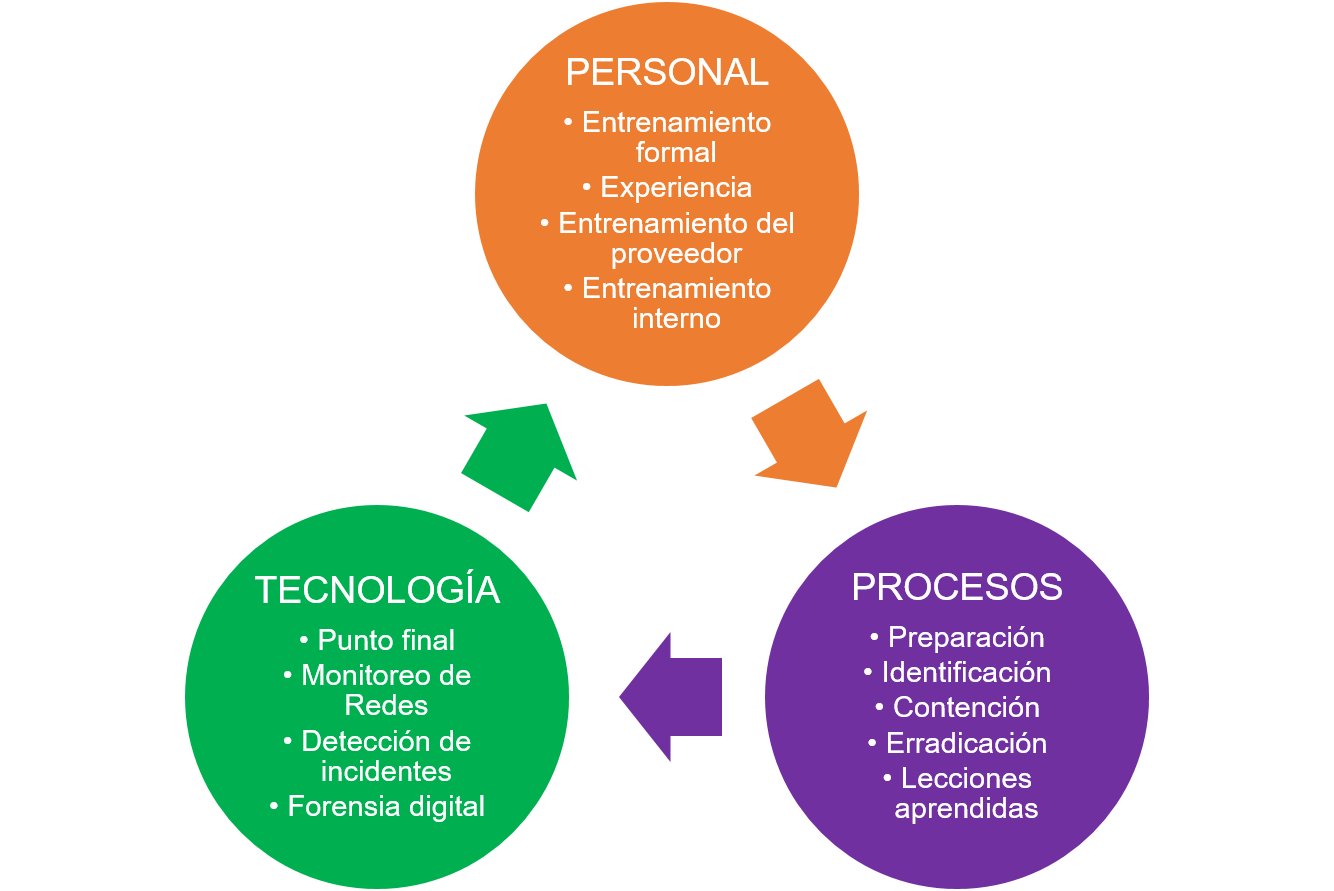
\includegraphics[width=1\textwidth]{./marco_teorico_imagenes/figura_1_pilares.png}
            \caption{Pilares de un CSIRT}
            \label{fig:pilares}
        \end{figure}
        %\par
        \FloatBarrier
        El CSIRT debe tener una perspectiva flexible y escalable para mantener el ritmo de las tácticas de los adversarios, acompañando el crecimiento y evolución de la organización. \par
    \end{section}
    
   \begin{section}{Personal}  
   En cuanto al personal, estos comprenden tanto a los encargados de dar respuesta a los incidentes como a los analistas del CSIRT. Si bien la propia organización puede designar a sus integrantes para asumir estas funciones, existen otras alternativas como la tercerización mediante empresas especializadas que proveen el servicio de Managed Security Service Provider (MSSP) o contratar especialistas en respuesta a incidentes en el caso de una emergencia o un problema complejo. Otra vía consiste en la creación de equipos híbridos compuestos por personal perteneciente a la organización y especialistas externos. \par
    De acuerdo a una encuesta del SANS Institute del año 2014 \cite{sans_1}, el 61\% de las organizaciones relevadas manifestaron haber recurrido a personal de emergencia para cubrir incidentes críticos y el 58 \% tenía un equipo de respuesta propio. Por lo que las organizaciones no siempre cubren sus necesidades con miembros de su propio personal y en algunos casos las tareas recaen por completo en los servicios de terceros. Esto se debe a que, sin importar la estructura del equipo, el personal de un CSIRT debe contar con el entrenamiento necesario para tratar con los cambios en las amenazas a las que se enfrenta. En el Cuadro \ref{table:1} se muestran las responsabilidades y la formación requerida para cada uno de los integrantes de un CSIRT. \par
    
    \begin{table}%[ht]
    \centering
        \begin{tabular}{ | m{10em} | m{16em}| m{11em} | } 
            \hline
            Título profesional & Tarea & Entrenamiento requerido \\ 
            \hline
            Nivel 1 - Analista de alertas & Supervisa continuamente la cola de alertas, monitorea el estado de los sensores y los puntos finales, clasifica las alertas de seguridad y recopila los datos necesarios para iniciar el trabajo de Nivel 2. & Procedimientos de triage de alerta y detección de intrusos. Gestión de redes, información de seguridad y eventos. Capacitación en investigación basada en host. \\ 
            \hline
            Nivel 2 - Analista de respuesta a incidentes & Realiza un análisis profundo de incidentes al correlacionar datos de varias fuentes y determina si un sistema crítico o un conjunto de datos se ha visto afectado. Asesora sobre su remediación. & Análisis avanzado de forensia de redes y basado en host. Procedimientos de respuesta a incidentes, revisiones de registros, evaluación básica de malware e inteligencia de amenazas. \\ 
            \hline
            Nivel 3 - Especialista en la materia & Se trata de un conjunto de especialistas que cubren distintas áreas de un CSIRT. 
            Actúan como “cazadores” de amenazas, sin esperar que se intensifiquen los incidentes. Se encuentra estrechamente involucrado en el desarrollo, ajuste e implementación de análisis de detección de amenazas.
             & Entrenamiento avanzado en detección de anomalías. Entrenamiento específico en herramientas para la agregación y análisis de datos e inteligencia de amenazas. 
            Poseen un conocimiento profundo en áreas como redes, puntos finales, inteligencia de amenazas, forensia e ingeniería inversa de malware, así como la infraestructura de IT subyacente.
            \\ 
             \hline
            Director del CSIRT & Administra recursos para incluir personal, presupuesto, programación de turnos y estrategias para cumplir con los acuerdos de nivel de servicio. Se comunica con la gerencia y sirve como persona de contacto en el caso de incidentes críticos. Proporciona una dirección general para el CSIRT. & Gestión de proyectos, formación en gestión de respuesta a incidentes, habilidades generales de gestión de personas y comunicación institucional.  \\
            \hline %linea final de tabla
        \end{tabular}
        \caption{Integrantes de un CSIRT y sus funciones}
        \label{table:1}
    \end{table}
    \FloatBarrier % obliga a la imagen a renderizarse antes de este punto
        Para organizar el trabajo de los analistas, un CSIRT necesita un director que coordine los múltiples esfuerzos dentro y fuera del equipo. Su responsabilidad es dirigir el trabajo y organizar los recursos con el fin de detectar, investigar y priorizar incidentes que puedan impactar en la organización. Otra de las misiones asignadas al director consiste en desarrollar un modelo de flujo de trabajo e implementar procedimientos operativos estandarizados, para el proceso de manipulación de incidentes, que guíen a los analistas en la clasificación y respuesta apropiada.
        En la Figura \ref{fig:org_csirt} se observa un modelo de organización de un CSIRT.
        
        \begin{figure}[H]
            \centering
            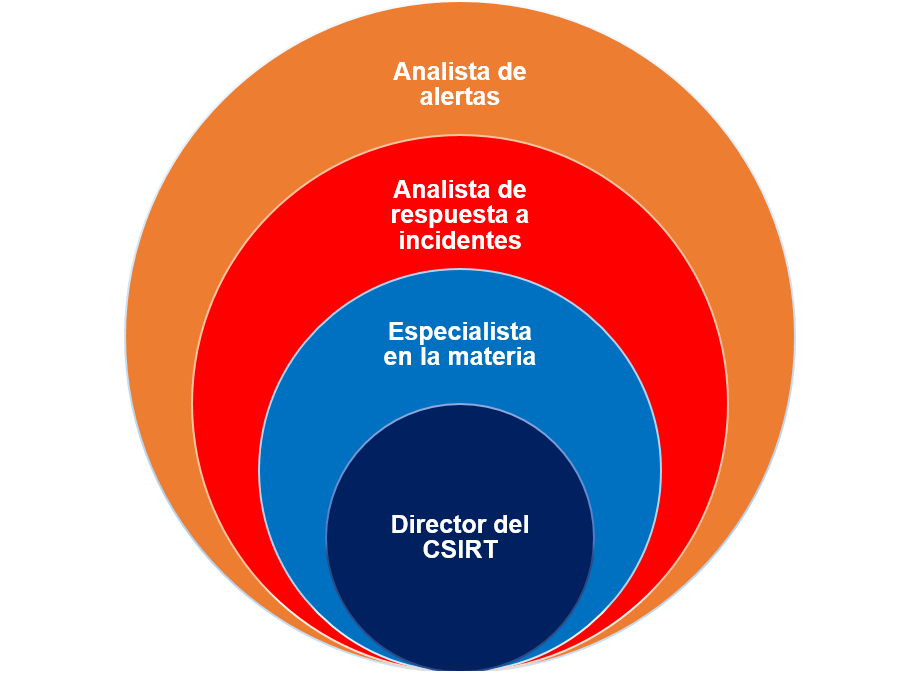
\includegraphics[width=1\textwidth]{./marco_teorico_imagenes/figura_2_org_csirt.png}
            \caption{Organización de un CSIRT}
            \label{fig:org_csirt}
        \end{figure}

   \end{section}
   
   \begin{section}{Procesos}  
        Para estandarizar las acciones que pueden tomar los analistas del CSIRT y asegurar que no se perderán tareas importantes en el camino, es necesario definir procesos repetibles de clasificación de incidentes e investigación. Al crear un flujo repetible de gestión de incidentes, se definen las responsabilidades y acciones de los miembros del equipo: desde la creación de una alerta y evaluación por analistas de nivel 1, hasta el tratamiento del incidente por parte del personal de los niveles superiores. Como consecuencia, la segmentación del proceso permite una gestión eficiente de los recursos del CSIRT. \par
    	Uno de los modelos de procesos de respuesta a incidentes más utilizado es el modelo DOE/CIAC \cite{doe_ciac}, que consiste en seis etapas: preparación, identificación, contención, erradicación, recuperación y lecciones aprendidas.

   \end{section}
   \begin{section}{Tecnología}
        En el núcleo de un CSIRT se encuentran las tecnologías de recolección de datos, agregación, detección, análisis y administración. En cuanto a la recolección, se trata de un sistema de monitoreo que obtiene sus datos a partir de un conjunto variado de fuentes como puntos finales (PC, dispositivos móviles, servidores, etc), redes, generadores de logs y eventos. Como resultado de la disponibilidad de los datos, antes y durante el incidente, los analistas pueden utilizar el sistema de vigilancia como una herramienta de investigación, revisando las actividades sospechosas del incidente en curso. Por otro lado, el sistema de monitoreo puede ser utilizado para generar la respuesta al incidente y potencialmente mitigar sus causas. \par
        Un aspecto importante a considerar es la compatibilidad de las tecnologías empleadas, en particular si la organización ya cuenta con una herramienta de monitoreo existente y se busca incorporar nuevas soluciones para integrarlas a los sistemas en servicio. En la Figura \ref{fig:comp_tech} se ejemplifica la necesidad de compatibilidad entre sistemas y componentes. 
        
        \begin{figure}[H]
            \centering
            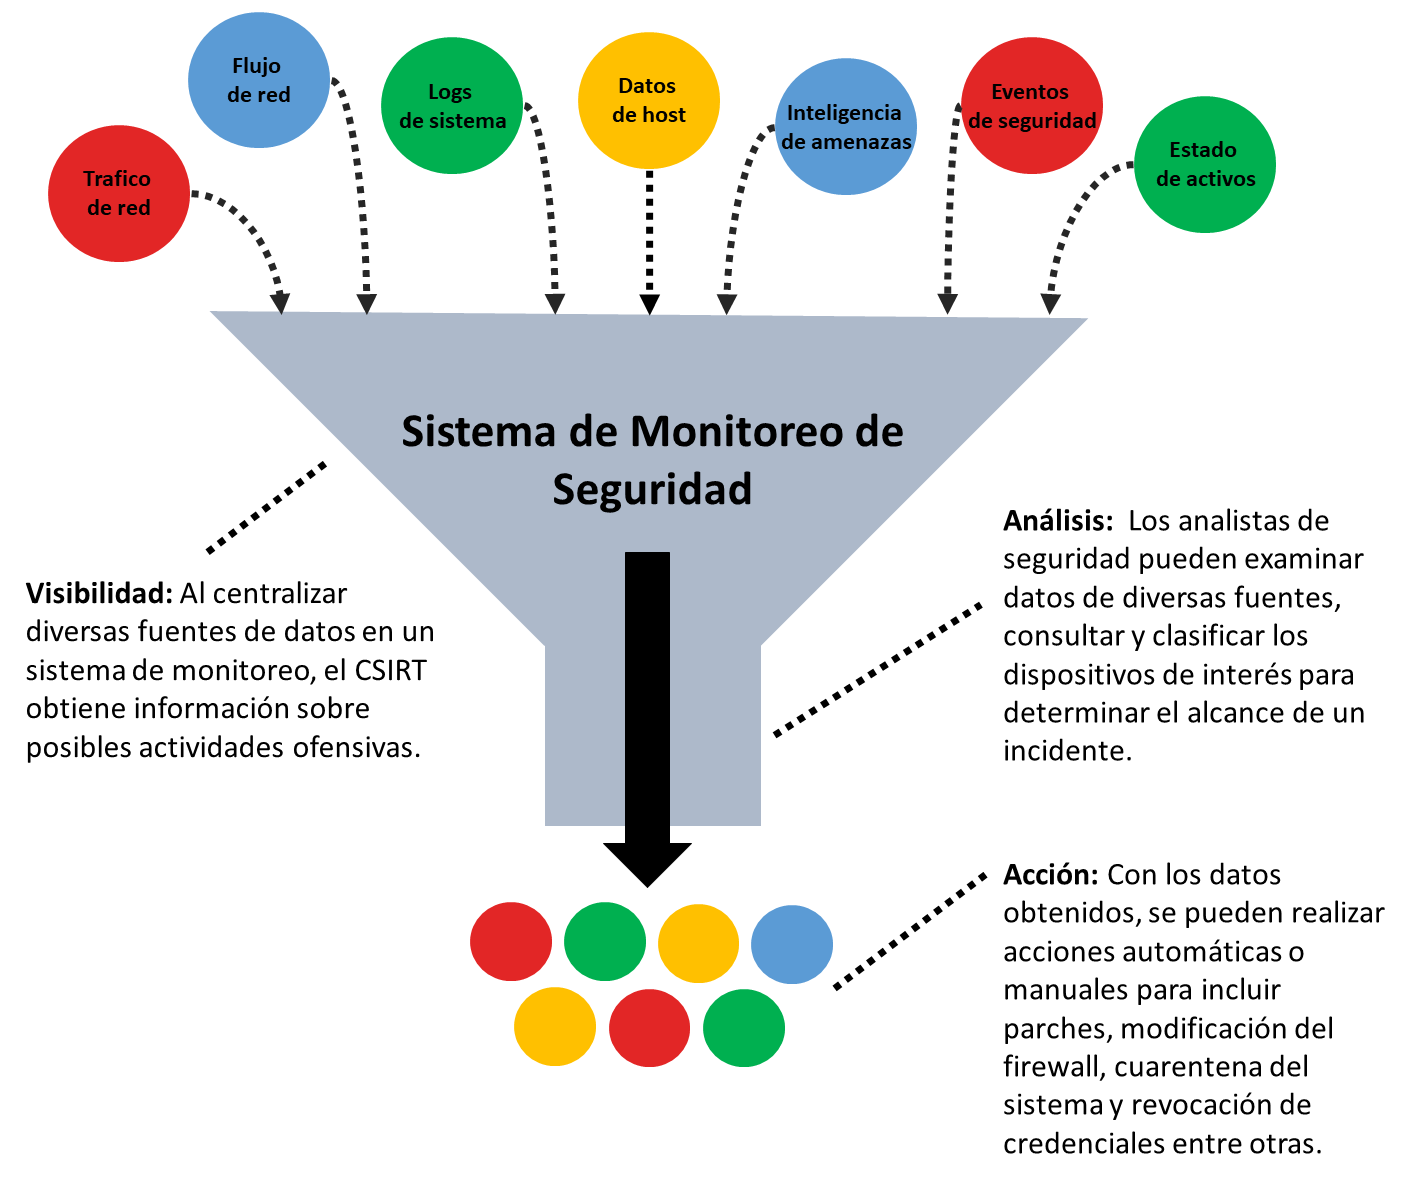
\includegraphics[width=1\textwidth]{./marco_teorico_imagenes/figura_3_compatibilidad_entre_tecnologias.png}
            \caption{Compatibilidad entre tecnologías de detección}
            \label{fig:comp_tech}
        \end{figure}
        \FloatBarrier
        \begin{subsection}{Agregando contexto a los incidentes}
        La incorporación de inteligencia de amenazas y otras informaciones de contexto tales como activos e identidades, contribuye al proceso de investigación del analista de un CSIRT. En determinados casos, la información inicial que está asociada a una alerta puede ser muy limitada, por ejemplo la dirección IP del punto final sospechoso es insuficiente por sí sola para tomar una decisión. \par
        Para que los analistas puedan investigar un incidente, generalmente necesitan más información, por ejemplo los nombres del dueño y de dominio de la máquina, registros DHCP para mapear la IP con el host al momento del incidente, etc. Si el sistema de monitoreo incorpora información de identidad y de los activos de información, entre otros datos de contexto, le permitirá al analista ahorrar tiempo y esfuerzo para priorizar los incidentes y elaborar la respuesta más apropiada.\par

        \end{subsection}
        \begin{subsection}{Definición de conductas normales}
        Dado que es posible observar patrones de comportamiento en usuarios, aplicaciones, infraestructura, redes y dispositivos, es útil establecer una referencia o línea base de la actividad de lo que se considerará un comportamiento normal. Esto facilitará la detección de conductas sospechosas anticipando posibles amenazas. \par
        Un sistema de monitoreo configurado y con una base de referencia adecuada estará en condiciones de enviar alertas confiables al analista de primer nivel. Esto obtiene especial relevancia, ya que de acuerdo al citado informe del SANS Institute del año 2014 \cite{sans_1}, uno de los principales desafíos en la utilización de registros de eventos de seguridad, es la incapacidad de distinguir actividades sospechosas de las normales. La ausencia de una referencia de “normalidad” es un obstáculo común al que se enfrentan las empresas de monitoreo y muchas organizaciones. \par
        La mejor práctica es utilizar plataformas que pueden crear líneas o patrones de referencia mediante el monitoreo de la red y la actividad de los puntos finales durante un periodo de tiempo.
        \end{subsection}
        
        \begin{subsection}{Inteligencia de amenazas}
        Los CSIRT bien establecidos o maduros desarrollan continuamente la capacidad de aprovechar la inteligencia de información proveniente tanto de sus incidentes pasados como de fuentes de inteligencia compartidas. Ejemplos de estas últimas son los proveedores especializados, CSIRT aliados, divisiones policiales de cibercrimen, organizaciones de intercambio de información como la Information Technology - Information Sharing and Analysis Center (IT-ISAC) \cite{it_isac}, etc. \par
        La capacidad de utilizar la inteligencia de amenazas contribuye a mejorar la precisión de la detección. De esta manera, es posible detectar patrones de amenazas ocultas en puntos finales, logs y registros de red, reduciendo las oportunidades de desarrollo de un ataque.
        \end{subsection}
        \pagebreak
        \begin{subsection}{Obstáculos para el manejo eficiente de incidentes del CSIRT}
        Algunos de los obstáculos que deben ser evitados por un CSIRT son aquellos que generan cuellos de botella en el proceso de respuesta a incidentes.  Este proceso que consiste en el traslado de un incidente entre los sucesivos niveles del CSIRT, eventualmente puede generar “ruido blanco”: la presencia de una gran cantidad de alertas de poca importancia y / o falsos positivos. De prolongarse esta situación en el tiempo, se produce un fenómeno llamado “fatiga de alertas” que afecta a los analistas provocando una disminución en sus capacidades de atender incidentes prioritarios. \par
        Al momento de elegir una herramienta de monitoreo, se debe considerar que incluya entre sus características la personalización del umbral de alertas y la posibilidad de combinar distintas alertas en un mismo incidente. Una herramienta de este tipo permite a los analistas clasificar las alertas más rápido, reduciendo las capas de evaluación necesarias antes de que el evento pueda ser confirmado y mitigado. 
        \end{subsection}
   \end{section}
      
   \begin{section}{Ámbitos de actuación de los CSIRT}
        En la actualidad existen en todo el mundo CSIRT pertenecientes a organizaciones que responden a distintos ámbitos de la sociedad y de diferente naturaleza (pública o privada). En términos generales, estos equipos se clasifican dependiendo de la comunidad a la que atienden, diferenciándose entre:
        \begin{itemize}
            \item \textbf{CSIRT para el sector de PYMES:} En este caso, el tamaño de las empresas hace poco viable que las organizaciones de este sector puedan implementar de forma individual las funciones de un CSIRT. Por lo tanto, surge la necesidad de unificar esfuerzos y servicios en un solo equipo capaz de dar soporte a varias empresas. La naturaleza de estos CSIRT puede ser pública o privada, dependiendo del contexto en el que se encuentren estas compañías.
            \item \textbf{CSIRT académico:} El área de responsabilidad de este tipo de equipos se circunscribe a instituciones académicas. Su tamaño, por lo tanto, puede variar dependiendo de las dimensiones de la comunidad, condicionando los servicios que ofrezcan, el modo en que lo hagan y su grado de intervención.
            \item \textbf{CSIRT comercial:} estos centros prestan distintos servicios a cambio de una contraprestación económica. Se trata de empresas especializadas en la industria de la ciberseguridad, que habitualmente utilizan acuerdos de servicios específicos con cada cliente.
            \item \textbf{CSIRT de proveedor:} se centra en los productos o servicios específicos de un proveedor. Su objetivo es proveer servicios y soluciones para eliminar o reducir el impacto negativo de las vulnerabilidades en estos últimos, ya sea un producto tecnológico o un servicio TIC.
            \item \textbf{CSIRT del sector militar:} Prestan servicios a organizaciones militares, con responsabilidades en infraestructuras TIC necesarias para la Defensa. Su comunidad está conformada por las instituciones militares y de entidades estrechamente relacionadas con éstas. Por ejemplo, en nuestro país el Comando Conjunto de Ciberdefensa \cite{fa_comando}, es el encargado de la defensa de la infraestructura de redes y activos de la información de las Fuerzas Armadas.
            \item \textbf{CSIRT para protección de infraestructuras críticas:}  Los CSIRT de este sector se centran principalmente en la protección de las infraestructuras críticas  y de los activos de información asociados. Ejemplos de infraestructuras críticas son las centrales y redes de energía, telecomunicaciones, sistema financiero, sector sanitario, agua, transportes, industria nuclear, etc.
            \item \textbf{CSIRT gubernamental:} Bajo esta denominación se sitúan los equipos cuyo principal objetivo es asegurar la infraestructura TIC de un Gobierno/Estado y los servicios ofrecidos a la población. La Comunidad a la que están dirigidos son las administraciones públicas y sus distintos organismos. Estos CSIRT gubernamentales generalmente forman parte de las instituciones del Estado.
            \item \textbf{CSIRT Nacional:} Este es un equipo con responsabilidad general de coordinación sobre todos los sectores y tiene una amplia responsabilidad sobre prácticamente todos los CSIRT tratados anteriormente. Este centro funciona como punto focal de contacto tanto en el entorno nacional como para requerimientos internacionales. ENISA, la Agencia de Ciberseguridad para la Unión Europea, define en un documento \cite{enisa} elaborado en diciembre de 2009, a este tipo de CSIRT como “aquel que actúa como el Point of Contact (POC) con otros equipos nacionales y/o internacionales. De hecho, podría considerarse como CSIRT  del último recurso, por su papel de coordinación”. Cada nación define la misión de estas unidades y establece sus operaciones, su organización y su imperativo legal en base a las necesidades del país y su comunidad. En Argentina, esta responsabilidad es asumida por la Dirección Nacional de Ciberseguridad \cite{dir_nac_ciber}. 
            \begin{figure}[H]
                \centering
              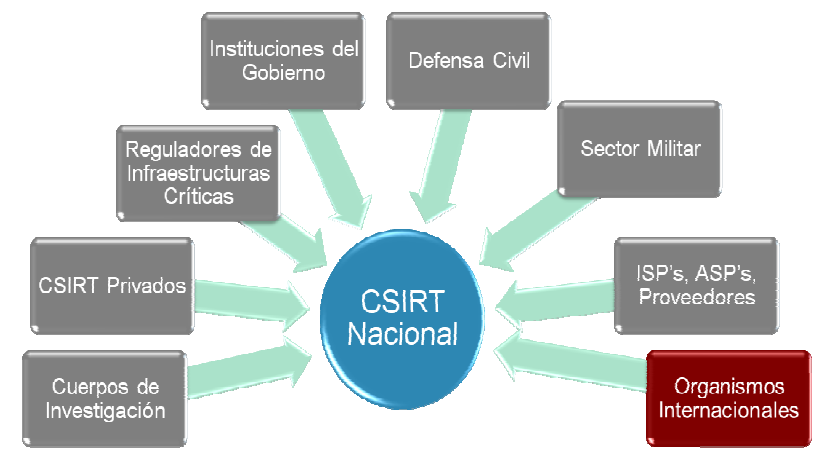
\includegraphics[width=0.8\textwidth]{./marco_teorico_imagenes/figura_4_csirt_nacional.png}
                \caption{CSIRT Nacional como centro de coordinación}
                \label{fig:csirt_nac}
            \end{figure}
            \FloatBarrier
            Frente a esto, todos los CSIRT nacionales tienen un objetivo común, mantener seguras las redes de sus países. De este modo podemos concluir que, aunque cada uno utiliza herramientas y procedimientos diferentes, todos comparten el mismo objetivo:
            \begin{enumerate}
                \item Designar un punto de contacto para la coordinación de la respuesta a incidentes.
                \item Construir y mantener una red de contactos extensa, tanto nacional como internacional.
                \item Monitorización de la situación actual y mejora de la concientización.
            \end{enumerate}
            Es importante destacar que la constitución de un CSIRT nacional o gubernamental, no es la única medida a tener en cuenta en una estrategia de ciberseguridad completa por parte de un Estado. Es una parte importante de la misma teniendo en cuenta, además, que este tipo de equipos deberían asumir la responsabilidad de la Protección de las Infraestructuras Críticas de Información (CIIP) del país.
        \end{itemize}
        \begin{subsection}{Estado de la ciberseguridad en Argentina} 
        Los orígenes de la gestión de la seguridad informática en nuestro país pueden rastrearse en el decreto 856/98 \cite{jef_gab_856_98} y a la Resolución de la Secretaría de la Función Pública (SFP), organismo dependiente de la Jefatura de Gabinete de Ministros, Res SFP 81/99 \cite{sub_tec}. Esta Resolución establece la reorganización de la Subsecretaría de Tecnologías Informáticas y el “Reglamento de Operación del ArCERT", donde se indican los requisitos y condiciones de operación de la Coordinación de Emergencia en Redes Teleinformáticas - ArCERT, y las Políticas de Seguridad del mismo. \par
        El objetivo principal del ArCERT fue coordinar y colaborar en los esfuerzos orientados a elevar los umbrales de seguridad en los recursos y en los sistemas de información en el ámbito de la Administración Pública Nacional (APN). Para esto se estableció una estrategia de coordinación, asesoramiento y capacitación hacia los organismos públicos en la gestión de la problemática de seguridad. \par
        Sus funciones \cite{sub_tec} eran: 
        \begin{enumerate}
            \item Proveer un servicio especializado de asesoramiento en seguridad de redes.
            \item Promover la coordinación entre los organismos de la Administración Pública Nacional para prevenir, detectar, manejar y recuperar incidentes de seguridad.
            \item Centralizar los reportes sobre incidentes de seguridad ocurridos en la APN y facilitar el intercambio de información para afrontarlos.
            \item Actuar como repositorio de toda la información sobre incidentes de seguridad, herramientas, técnicas de protección y defensa.
        \end{enumerate}
        En el marco de las funciones nombradas, el ArCERT realizó actividades de investigación de amenazas y nuevas soluciones disponibles,  divulgación de incidentes y soluciones así como capacitaciones de seguridad en redes y seminarios de actualización periódicos. \par
        El año 2011 marcó el comienzo de un largo proceso de reestructuración de los organismos del Estado Nacional relativos a la ciberseguridad, que incluyó el reordenamiento de estructuras internas, la creación de nuevas dependencias y el reemplazo o absorción de unidades preexistentes por las de nueva formación. Ese mismo año, mediante la resolución de la Jefatura del Gabinete de Ministros, Res JGM Nº 580/2011 \cite{jef_gab_crease} se creó el Programa de Infraestructuras Criticas de Informacion y Ciberseguridad, que declaró como finalidad “Impulsar la creación y adopción de un marco regulatorio específico que propicie la identificación y protección de las Infraestructuras estratégicas y críticas del Sector Público Nacional, los organismos interjurisdiccionales y las organizaciones civiles y del sector privado que así lo requieran”. \par
        En el año 2013 y mediante el artículo 1º de la Disposición Nº 2/2013 \cite{disp_2_2013} de la Oficina Nacional de Tecnologías de Información (ONTI), se creó el Instituto de Ciencias e Ingeniería de Computación - Computer Emergency Response Team (ICIC-CERT) que reemplazó al ArCERT. \par
        Este nuevo CERT heredaba parte de las responsabilidades del original, a la par que otros artículos de la referida disposición creaban nuevos grupos de trabajo especializados que ampliaban las capacidades, funciones y responsabilidades concentradas originalmente en el ArCERT, tales como el grupo ICIC - GAP (Grupo de Acción Preventiva, art. 3º) con funciones similares a las encargadas al ArCERT pero enfocadas a monitorear “los servicios que el Sector Público Nacional brinda a través de la red de Internet y aquellos que se identifiquen como Infraestructura Crítica para la prevención de posibles fallas de Seguridad”, el grupo “ICIC - GICI” (Grupo de Infraestructuras Críticas de Información, art. 4º) especializado en el desarrollo y aplicación de nuevas tecnologías para el monitoreo, simulación y respuesta a incidentes en la red de infraestructuras críticas, establecer prioridades y planes estratégicos para liderar el abordaje de la ciberseguridad para la protección de este tipo de infraestructuras, coordinar la implementación de ejercicios de respuesta ante la eventualidad de un intento de vulneración de estos activos, entre otras. Finalmente, se creó el grupo de trabajo “ICIC - INTERNET SANO” (art. 7º) con el objetivo específico de ocuparse de las tareas de difusión y capacitación que anteriormente le correspondía al ArCERT. En cuanto al programa de infraestructuras críticas, podemos mencionar la adhesión de la Universidad Nacional de Córdoba, cuando el 15 de Julio de 2014, mediante la Resolución 1221 \cite{unc_rec} firmada por el Rector Tamarit, en su artículo N°1 “Hacer lugar a lo solicitado a fS.1 por la Prosecretaría de Informática y, en consecuencia, adherir al "Programa Nacional de Infraestructuras Críticas de Información y Ciberseguridad"...” \par
        El Estado Nacional siguió actualizando sus políticas en los años siguientes, creando nuevos centros de respuesta a incidentes y actualizando la normativa vigente. Algunos de los ejemplos son la creación del Comando Conjunto de Ciberdefensa de las Fuerzas Armadas \cite{fa_comando}, el “MING-CSIRT” \cite{minis_seg} del Ministerio de Seguridad de la Nación, la Dirección Nacional de Ciberseguridad \cite{dir_nac_ciber} y sus correspondientes unidades de gobierno. \par
       \begin{figure}[H]
            \centering
            \subfloat[\centering] {{
\includegraphics[width=5 cm, valign=c]{./marco_teorico_imagenes/figura_5a_comando_conjunto.png}}} %
            \quad
            \subfloat[\centering] {{
\includegraphics[width=5 cm, valign=c]{./marco_teorico_imagenes/figura_5b_csirt_neuquen.png}}} %
            \caption{Insignias de CSIRTS argentinos: (a) corresponde al Comando Conjunto de Ciberdefensa y (b) corresponde al CSIRT de la provincia de Neuquén}
            \label{fig:ciberdef_nqn}
        \end{figure}
        \FloatBarrier
        Por otro lado, los Estados Provinciales, universidades y empresas también han desarrollado e implantado CSIRTs en sus organizaciones. Algunos ejemplos de esto son el “BA-CSIRT”\cite{ba_csirt} de la Ciudad de Buenos Aires, el “CSIRT-NQN”\cite{nqn_csirt} del gobierno de la provincia de Neuquén, “CERT UNLP” \cite{unlp_cert} de la Universidad Nacional de La Plata o el que dispone NIC Argentina \cite{nic_arg} destinado a la infraestructura crítica de DNS. En el caso de las empresas, podemos mencionar a los CSIRT de las redes bancarias Link \cite{red_link} y Banelco\cite{banelco}.
            \begin{subsubsection}{Demanda de ciberseguridad Argentina}
            Nuestro país, de manera análoga a los demás países de la región, ha experimentado un crecimiento exponencial de incidentes de ciberseguridad a lo largo de las últimas dos décadas. Esto afecta a individuos, empresas, universidades, infraestructuras críticas y a los organismos de diferentes niveles del gobierno. Este incremento exponencial en la demanda de ciberseguridad no ha encontrado una respuesta adecuada del Estado Argentino. Un ejemplo lo constituyen los 1590 millones de ataques \cite{iProUP} que sufrió el sistema bancario argentino en el año 2019 o los 187 millones de ciberataques entre enero y marzo del 2020 con un incremento del 131\% solo para el mes de marzo, según la plataforma “Fortinet Threat Intelligence Insider Latin America” \cite{fortinet}. \par 
            En la Figura \ref{fig:cant_intentos} se observan las diez amenazas más frecuentes y la cantidad de ataques producidos en Argentina por ellas, en el periodo comprendido entre los meses de abril y junio de 2020. Los tres primeros corresponden al troyano de puertas traseras “DoublePulsar Backdoor”, negociación de cifrados SSL anónimos e intentos de ataque contra una vulnerabilidad de divulgación de información en el servidor SMB de Microsoft Windows. La fuente es un informe de Fortinet Threat Intelligence Insider Latin America \cite{fortinet}.\par
            \begin{figure}[H]
            \centering
            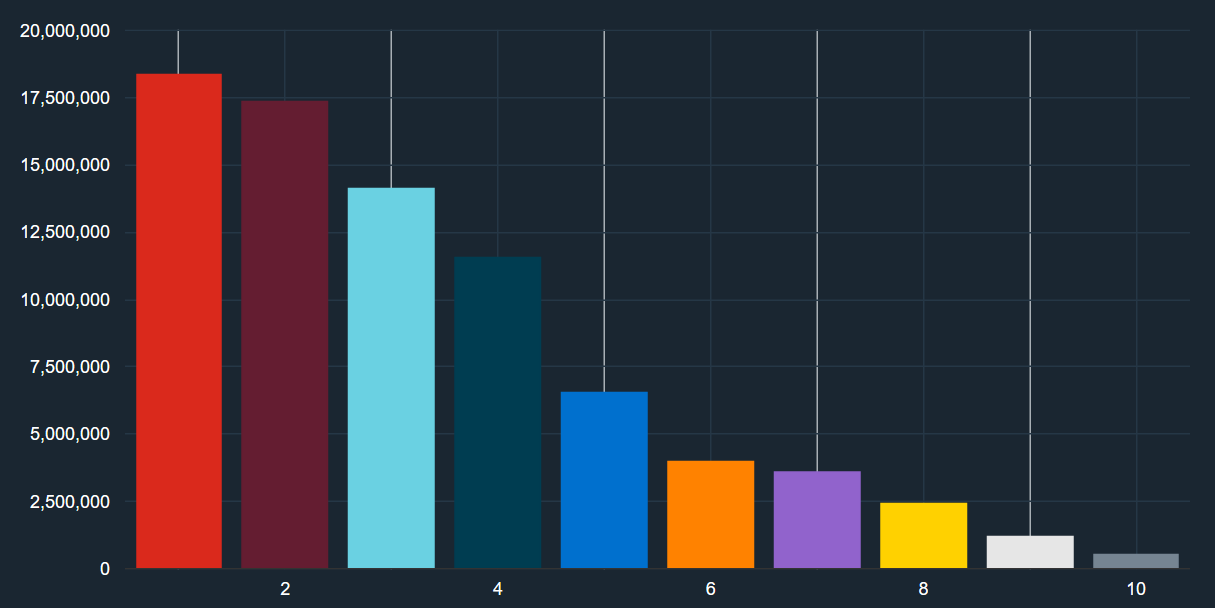
\includegraphics[width=1\textwidth]{./marco_teorico_imagenes/figura_6_cant_intentos_intrusion.png}
            \caption{ Cantidad de intentos de intrusión según la amenaza. Abril - Junio de 2020}
            \label{fig:cant_intentos}
        \end{figure}
        \FloatBarrier
        Hay informes del gobierno nacional \cite{panorama} disponibles desde el 2016 que anticipan esta tendencia, en particular el Ministerio de Modernización indicó que el país registró 5.400 millones de dólares en pérdidas atribuidas a incidentes de ciberseguridad. Esto representa el 1\% del PBI \cite{pbi} del mismo año. La Figura \ref{fig:porcentaje_tipos} del mencionado informe muestra los tipos de incidentes más frecuentes del año 2016 \par
        \begin{figure}[H]
            \centering
            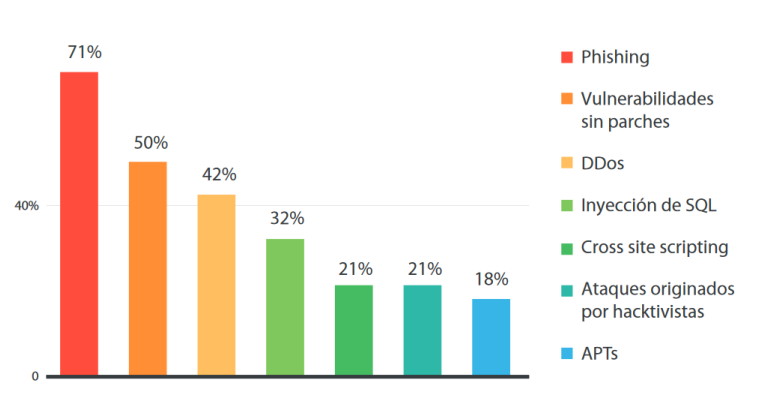
\includegraphics[width=1\textwidth]{./marco_teorico_imagenes/figura_7_tipos_de_incidentes.png}
            \caption{Porcentaje de tipos de incidentes durante 2016}
            \label{fig:porcentaje_tipos}
        \end{figure}
        \FloatBarrier
        Este costo, enorme tanto en relación a la producción nacional como en forma cuantitativa, resalta la necesidad cada vez más importante de desarrollar políticas públicas activas en forma de inversiones en la ampliación de las capacidades de análisis y respuesta a amenazas de ciberseguridad en los organismos de la Administración Pública. \par
        Resulta por lo tanto, necesaria la promoción de iniciativas privadas junto a la concientización de los riesgos existentes, el fomento de investigaciones académicas y la formación de recursos humanos capaces de afrontar estos desafíos, junto a una legislación adecuada y actualizada, para responder al constante aumento de amenazas y complejos escenarios que implica la creciente actividad en línea de industrias, organismos del Estado, comercio y desarrollo de la sociedad en Internet. \par

            \end{subsubsection}
        \end{subsection}
   \end{section}

    \begin{section}{SIEM: Definición y funciones}
    Las capacidades que ofrece un CSIRT para las organizaciones, en términos de prevención y mitigación de incidentes informáticos, se basan en los tres pilares mencionados en las secciones anteriores: el personal, la tecnología y los procesos. \par
    En cuanto a la tecnología, es la que permite llevar a cabo las tareas de recolección de datos, agregación, detección, análisis y administración. Estas tecnologías se encuentran dentro del marco operacional del Security Information and Event Management (SIEM) como entidad dentro de la estructura de organización de un CSIRT. \par
    El proceso de monitoreo de la seguridad de una red de datos compleja requiere recopilar diferentes tipos de datos para detectar, verificar y contener acciones ofensivas. Las tecnologías del SIEM proporcionan informes en tiempo real y análisis de eventos de seguridad a largo plazo, como se muestra en la Figura 8. Todo esto ayuda a la tarea de un analista de ciberseguridad cuando debe verificar acciones ofensivas sobre la red de una organización. \par
    El término SIEM fue acuñado en 2005 por los analistas Amrit Williams y Mark Nicolett de la compañía estadounidense Gartner \cite{def_siem}, una empresa especializada en investigación y consultoría de incidentes de seguridad, unificando los acrónimos en inglés SIM (security information management) y SEM (security events management) para describir metodologías muy similares pero ligeramente diferentes de ciberseguridad. Esta superposición de tareas hizo evidente que un nuevo término podría englobar ambos conjuntos de funciones, con el fin de disponer de un único acrónimo que pudiese identificar a una plataforma capaz de resolver los objetivos de los sistemas predecesores. \par
    De esta manera, el nuevo acrónimo SIEM significa Administración de Eventos de Seguridad de la Información, por sus siglas en inglés. Como plataforma que combina las funciones de los sistemas anteriormente descritos, sus capacidades comprenden la siguiente lista de tareas:
    \begin{itemize}
        \item Recolectar, analizar y presentar de manera eficiente datos relacionados a la seguridad.
        \item Análisis en tiempo real de eventos de seguridad.
        \item Generar reportes y almacenar datos relacionados a la seguridad.
        \item Administración de niveles y tipos de acceso e identidad.
        \item Auditoría de registros.
        \item Respuesta a incidentes y operaciones de seguridad.
    \end{itemize}
    Como se puede observar en la Figura \ref{fig:flujo_datos_siem}, para cumplir con las tareas anteriormente descritas, un SIEM obtiene su información de diversas fuentes:
    \begin{itemize}
        \item Inteligencia de Amenazas, identidades y logs: la revisión de amenazas pasadas y la inteligencia compartida por otras organizaciones aliadas contribuyen a detectar más rápido patrones anormales de comportamiento.
        \item Telemetría de Netflow: es un protocolo de recopilacion de informacion del flujo de red IP.
        \item Captura de paquetes: replicación de paquetes de información con el fin de correlacionar posibles amenazas en el flujo de red.
        \item Dispositivos Antimalware: componentes especializados en la detección de malware, localizados en puntos finales.
        \item IDS (HIDS y NIDS): Sistemas de detección de intrusiones, orientados a redes (NIDS) o puntos finales (HIDS).
        \item Firewalls: software que bloquea y filtra conexiones con origen desde el sistema hacia el exterior y viceversa.
        \item IPS: Sistema de protección de intrusiones. Ofrecen protección activa frente a comportamientos inusuales ya que pueden tomar acciones programadas para evitar un intento de intrusión.
        \item Syslog: Syslog es un protocolo para el tratamiento de logs en un formato estandarizado, empleado fundamentalmente en el monitoreo de la integridad de servidores.
    \end{itemize}
      \begin{figure}[H]
            \centering
            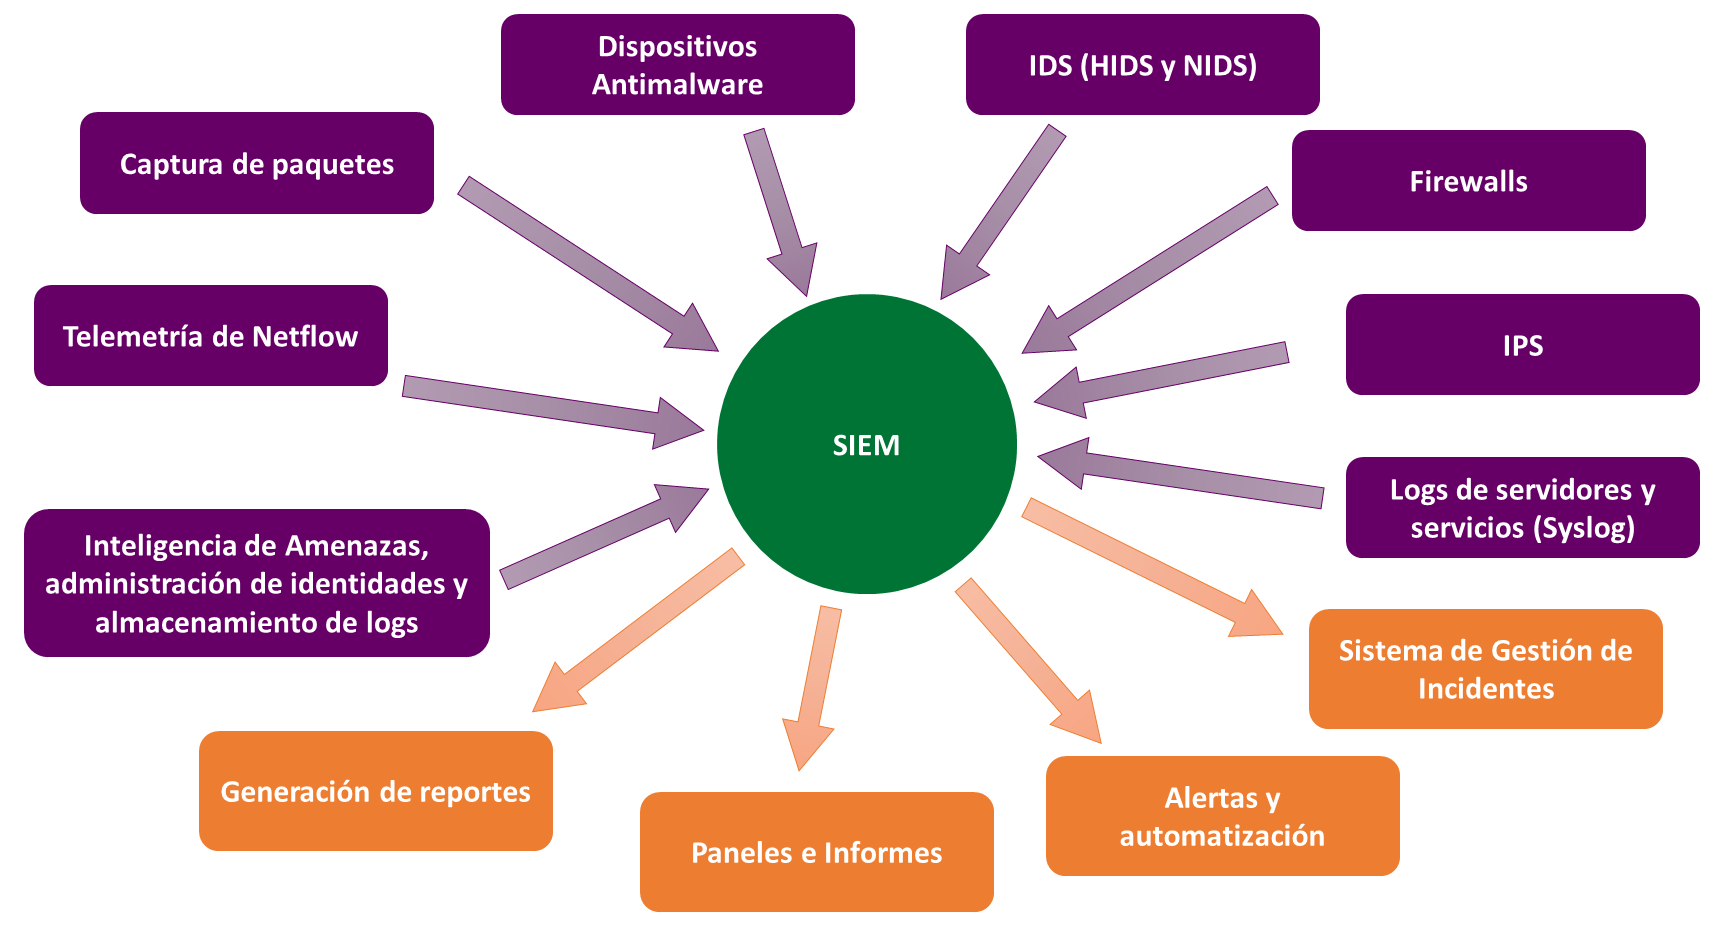
\includegraphics[width=1\textwidth]{./marco_teorico_imagenes/figura_8_datos_de_un_siem.png}
            \caption{Funciones y flujos de datos de un SIEM}
            \label{fig:flujo_datos_siem}
        \end{figure}
        \FloatBarrier
        La secuencia del tratamiento que recibe la información dentro un SIEM está representada en la Figura \ref{fig:procesos_siem}, donde se muestran los cuatro pasos que forman el proceso de respuesta a incidentes del SIEM. La secuencia se detalla a continuación:
        \begin{itemize}
            \item Paso 1: inicialmente es necesario recolectar datos provenientes de diversas fuentes, tales como sistemas IDS, firewall, syslog, switches (protocolos SNMP), entre otros. Como estos datos tienen formatos disímiles entre sí, es necesario un posterior proceso de normalización.
            \item Paso 2: a medida que los datos arriban al SIEM, es necesario someterlos a un proceso de normalización. Este proceso consiste en extraer la información contenida en los distintos mensajes, para almacenarla en un formato estandard. Con el objetivo de reducir el volumen de almacenamiento, la información resultante es sometida a un proceso de agregación, que separa los datos importantes de los secundarios.
            \item Paso 3: es posible analizar los datos resultantes en busca de patrones de actividad inusual. Esta búsqueda se puede realizar de manera manual por un analista o en forma autónoma en el caso de disponer de herramientas  que utilicen inteligencia de amenazas.
            \item Paso 4:  con los resultados del análisis del paso anterior, es posible determinar la existencia de un intento de intrusión u otros tipos de incidentes. De confirmarse este último caso, es posible enviar alertas a los responsables de tomar decisiones para mitigar el incidente.
        \end{itemize}
    \begin{figure}[H]
            \centering
            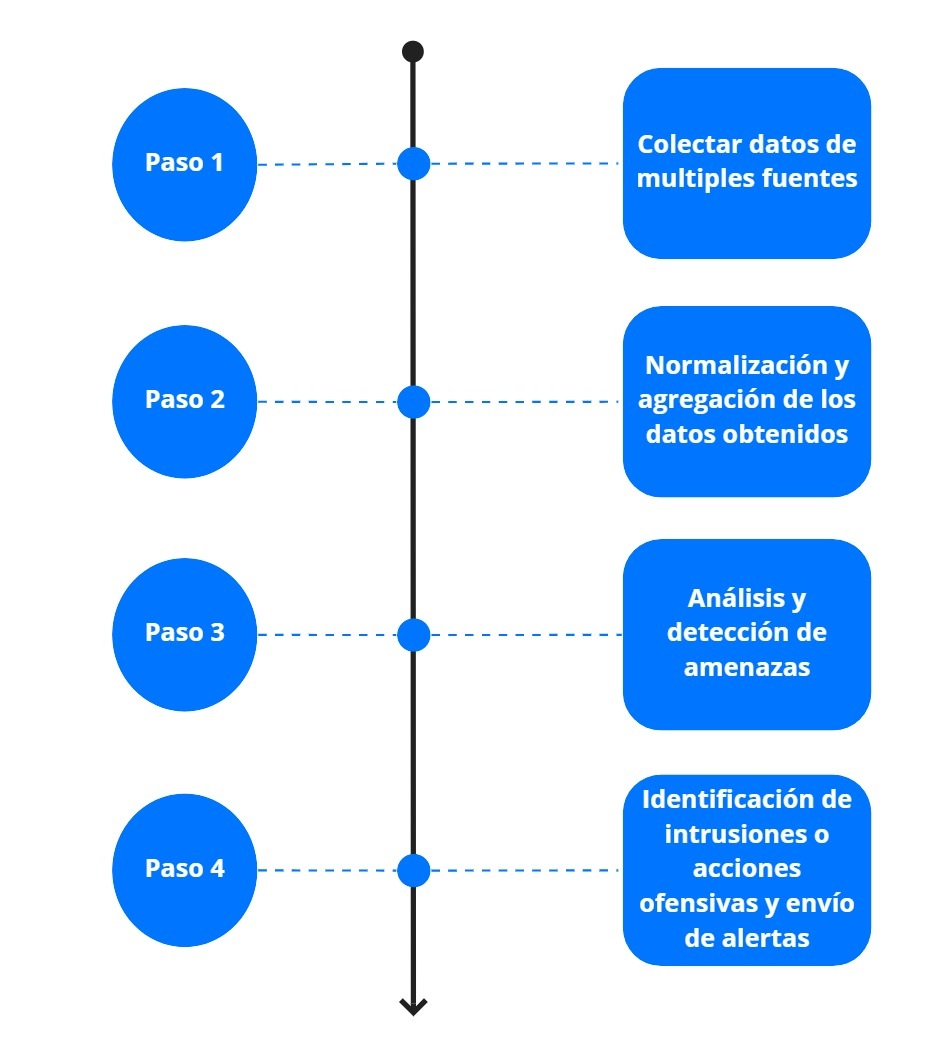
\includegraphics[width=1\textwidth]{./marco_teorico_imagenes/figura_9_procesos_de_un_siem.jpg}
            \caption{Proceso de identificación y respuesta a incidentes de un SIEM}
            \label{fig:procesos_siem}
        \end{figure}
        \FloatBarrier    
        El objetivo, por lo tanto, de un sistema SIEM dentro del CSIRT es concentrar la información proveniente de múltiples fuentes independientes, procesar los datos y realizar un análisis centralizado.
    \end{section}
    \pagebreak
    \begin{section}{Soluciones disponibles}
    Las principales soluciones que existen en el mercado, sean gratuitas, de software libre, pagas o de código propietario,  se presentan a continuación.\par
    En primer lugar se realizó un relevamiento en sitios especializados y de referencia para el mercado mundial, con el objetivo de identificar las soluciones comerciales disponibles, que actualmente dominan el mercado global de SIEM . En el sitio web de Gartner \cite{ranking} se encontró un listado de los productos ordenados por valoración de los usuarios de dicha página. El resultado de los diez primeros productos junto a sus desarrolladores, se muestra en el Cuadro \ref{table:2}. \par
    \begin{center}
        \begin{table}[H]
        \centering
        \begin{tabular}{ | m{4em} | m{22em}| m{12em} | }
            \hline
            Posición & Nombre de la solución & Empresa desarrolladora \\ 
            \hline
            1) & QRadar SIEM\cite{qradar} & IBM. \\ 
            \hline
            2) & ManageEngine ADAudit Plus\cite{adaudit} & ManageEngine. \\ 
            \hline
            3) & LogRhythm NextGen SIEM Platform\cite{logrhythm}
             & LogRhythm
            \\ 
             \hline
            4) & LogPoint - SIEM\cite{logpoint} & LogPoint  \\
             \hline
            5) & McAfee Enterprise Security Manager\cite{enterprise} & McAfee  \\
             \hline
            6) & ArcSight Enterprise Security Manager (ESM)\cite{arcsight} & Micro Focus  \\
             \hline
            7) & InsightIDR\cite{insight} & Rapid7  \\
             \hline
            8) & Elastic (ELK) Stack\cite{elastic} & Elastic  \\
             \hline
            9) & Splunk Enterprise\cite{splunk} & Splunk  \\
             \hline
            10) & Exabeam Security Management Platform\cite{exabeam} & Exabeam \\
            \hline %linea final de tabla
        \end{tabular}
        \caption{Ranking Gartner \cite{ranking} de soluciones SIEM 2020}
        \label{table:2}
    \end{table}
    \end{center}
    \FloatBarrier
    En base a la información recolectada, se procedió a clasificar las herramientas bajo el criterio de la disponibilidad del código: propietarias o libres y el resultado se muestra en el Cuadro \ref{table:3}.
        \begin{table}[h]
        \begin{tabular}{ | m{22em}| m{17em} | } 
            \hline
            Soluciones Pagas y Propietarias & Soluciones Libres y Gratuitas  \\ 
            \hline
            Splunk\cite{splunk} &  \\ 
            
            McAfee Enterprise Security Manager\cite{enterprise} &  \\
            
            AlienVault USM\cite{alienvault_usm} & Graylog\cite{graylog} \\ 
             
            QRadar SIEM \cite{qradar} & Elastic (ELK) Stack\cite{elastic}  \\
             
            ManageEngine ADAudit Plus\cite{adaudit} & AlienVault OSSIM\cite{alienvault_ossim}  \\
             
            LogRhythm NextGen SIEM Platform\cite{logrhythm} & Security Onion\cite{sonion}  \\
             
            LogPoint - SIEM\cite{logpoint} & Sweet Security\cite{sweet_security}  \\
             
            ArcSight Enterprise Security Manager (ESM)\cite{arcsight} &   \\
             
            InsightIDR\cite{insight} &   \\
             
            \hline %linea final de tabla
        \end{tabular}
        \caption{Ranking Gartner \cite{ranking} de soluciones SIEM 2020}
        \label{table:3}
    \end{table}
    
    \pagebreak
    
    \begin{subsection}{Soluciones comerciales}
    
        En nuestro análisis de las soluciones comerciales disponibles, se decidió describir la situación del mercado internacional en función de los siguientes criterios: 
        Usuarios (descritos a través de los sectores industriales a los que pertenecen), la distribución geográfica de los usuarios a nivel global y luego repetimos el análisis con un énfasis en América Latina. \par 
        Respecto de los sectores industriales que hacen uso de sistemas de ciberseguridad y generan demandas de nuevas soluciones, se observó que el sector financiero a nivel mundial es el que lidera el consumo de soluciones SIEM, con la mayoría de los desarrolladores teniendo como clientes principales a empresas y organizaciones de este sector. Esto se explica dado el alto nivel de digitalización de la banca y los servicios financieros, que por su masividad y naturaleza son objetivos prioritarios para cualquier atacante en el ciberespacio. \par
        Finalmente, se hizo una comparación por características entre los principales productos SIEM del mercado internacional, en base a las revisiones de sus usuarios en distintos medios, en particular se tuvo referencia a las publicaciones de “Gartner”\cite{ranking} y “Markets \& Markets”\cite{markets_markets}. 
        Los resultados se encuentran en la Figura \ref{fig:tabla_valoracion}.\par
        %\textfloatsep
        \protect
         \begin{figure}
            \centering
            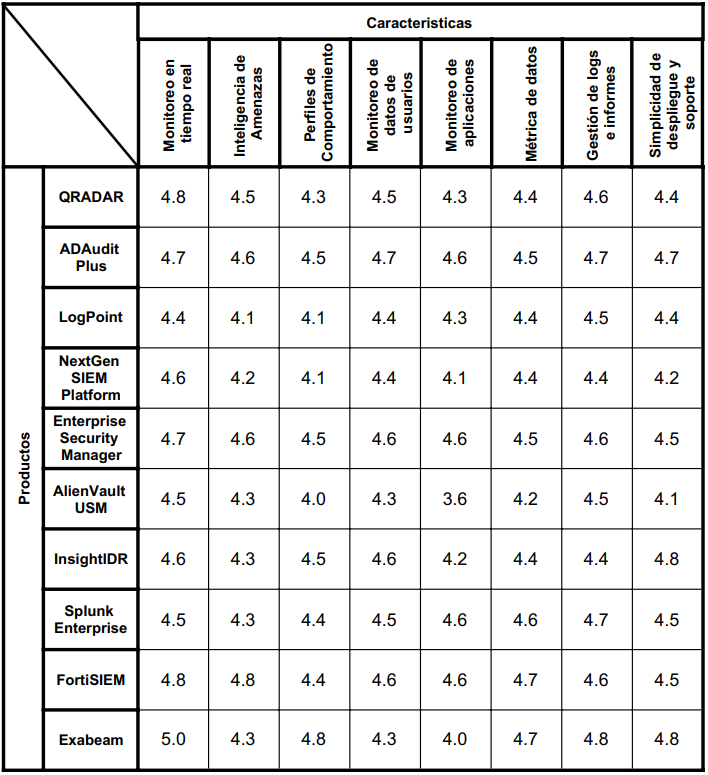
\includegraphics[width=1\textwidth]{./marco_teorico_imagenes/tabla_3_valoracion.png}
            \caption{Valoración de las características}
            \label{fig:tabla_valoracion}
        \end{figure}
        \FloatBarrier
        En la figura comparativa \ref{fig:tabla_valoracion} se observó que FortiSIEM y ADAudit Plus, de las compañías Fortinet\cite{fortisiem} y ManageEngine\cite{adaudit} respectivamente, son las soluciones mejor valoradas.
        \begin{figure}[H]
        \centering
        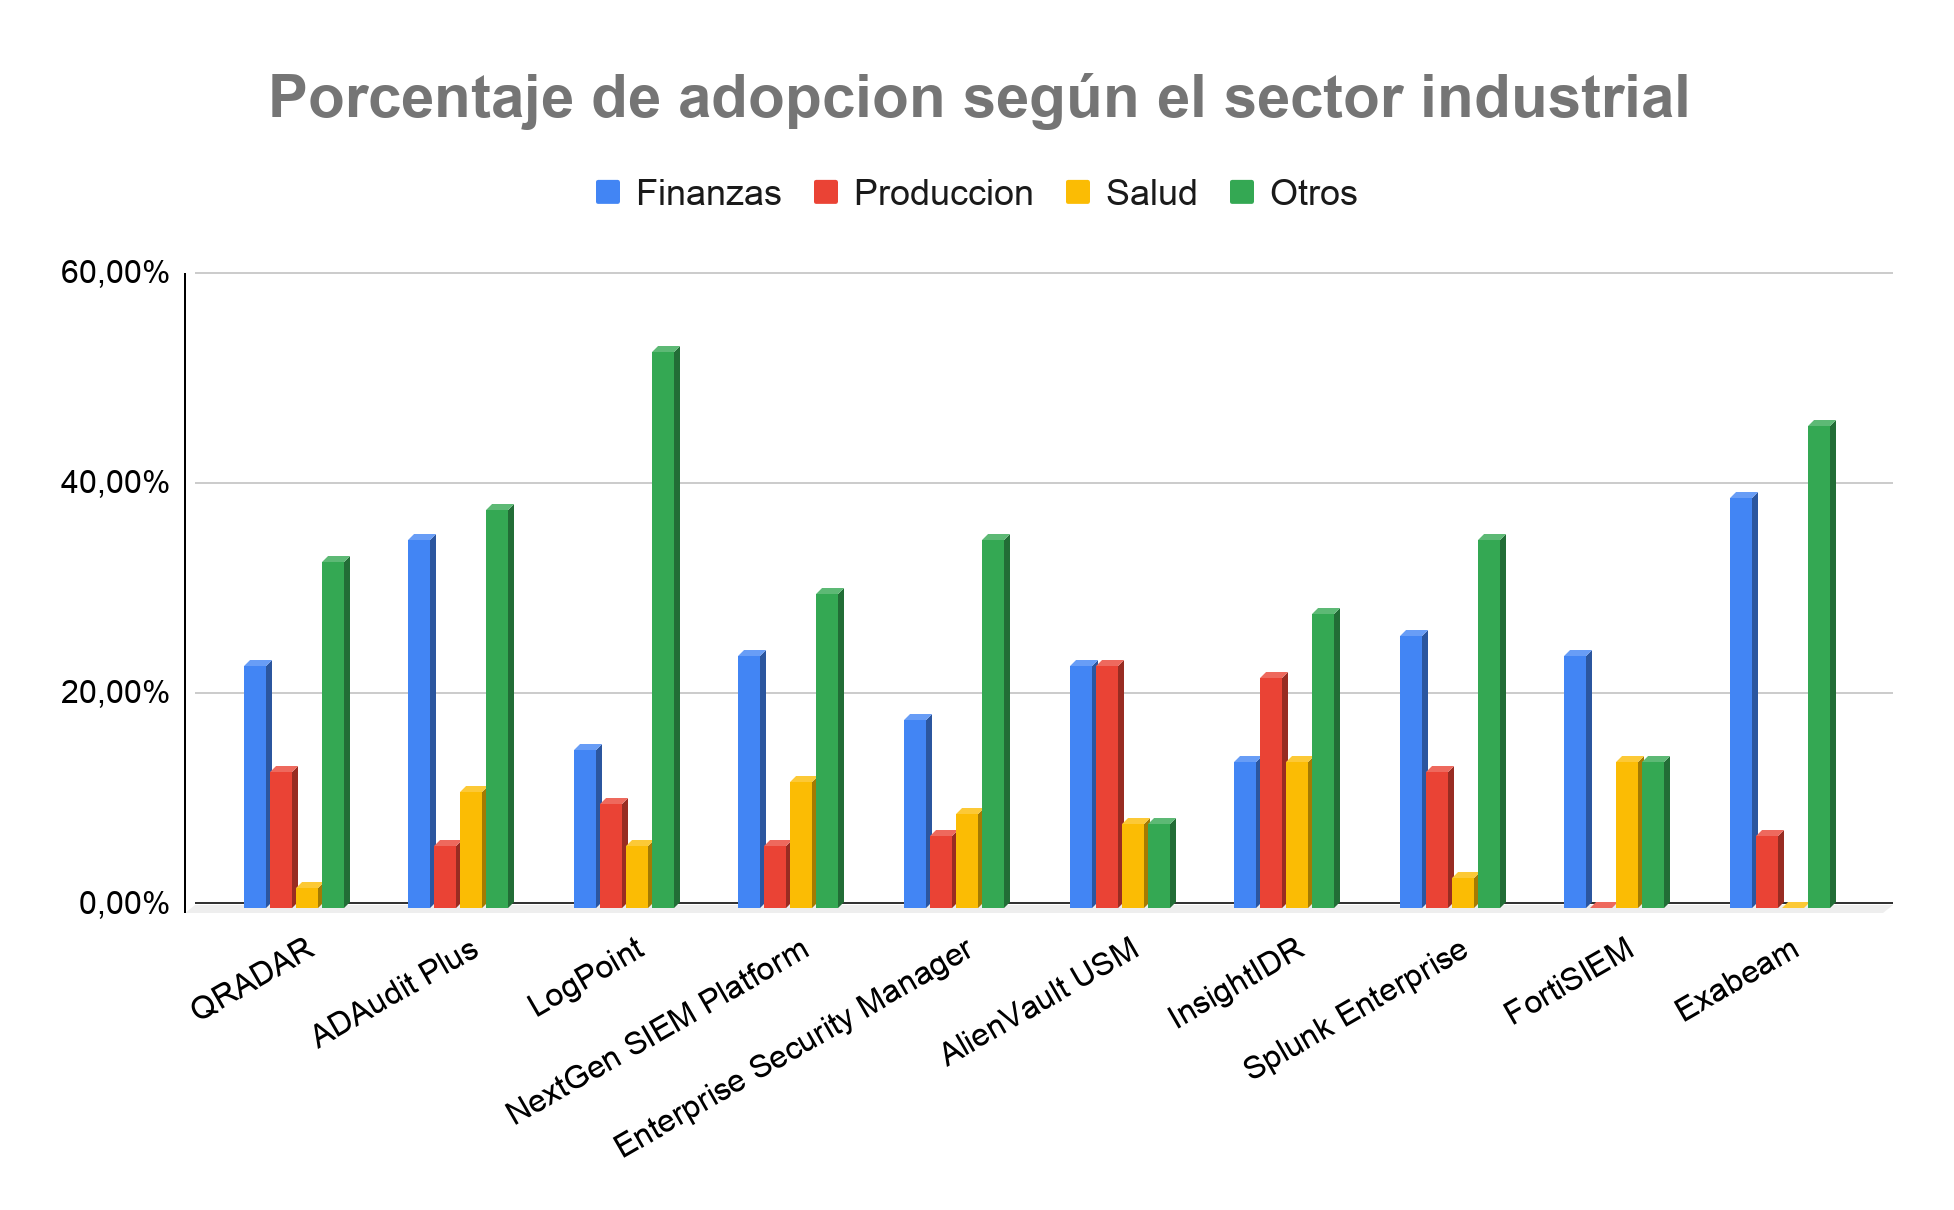
\includegraphics[width=1\textwidth]{./marco_teorico_imagenes/figura_10_porcentaje_sector_ind.png}
        \caption{Porcentaje de adopción según el sector industrial}
        \label{fig:sector_industrial}
        \end{figure}
        \FloatBarrier
       
        En las Figuras \ref{fig:sector_industrial} y \ref{fig:area_geografica_mundial} se aprecia que el sector financiero es el principal demandante de estas soluciones a nivel global, seguido por las industrias manufactureras y de salud. Los sectores industriales se destacan con diferencia respecto al resto en términos de adopción de soluciones SIEM. Esto se debe a que la automatización de la industria primero y su evolución al actual modelo de “industrias 4.0” \cite{industrias_4}, con cadenas de producción, montaje y ensamble distribuidas geográficamente alrededor del globo, implica uso masivo de sensores, redes y datos intrínsecos a cada fase de producción. Esto produjo la necesidad de contar con soluciones de ciberseguridad para evitar incidentes que impliquen el posible robo de información crítica o secretos industriales. De manera análoga al sector manufacturero, las clínicas, hospitales \cite{CCN_CERT} y centros de salud han sufrido el impacto de la digitalización de sus procesos tanto en el hardware médico, el almacenamiento y distribución de la información como en la protección de los sensibles datos privados de los pacientes y la estricta normativa que los regula. \par
        \begin{figure}[H]
            \centering
            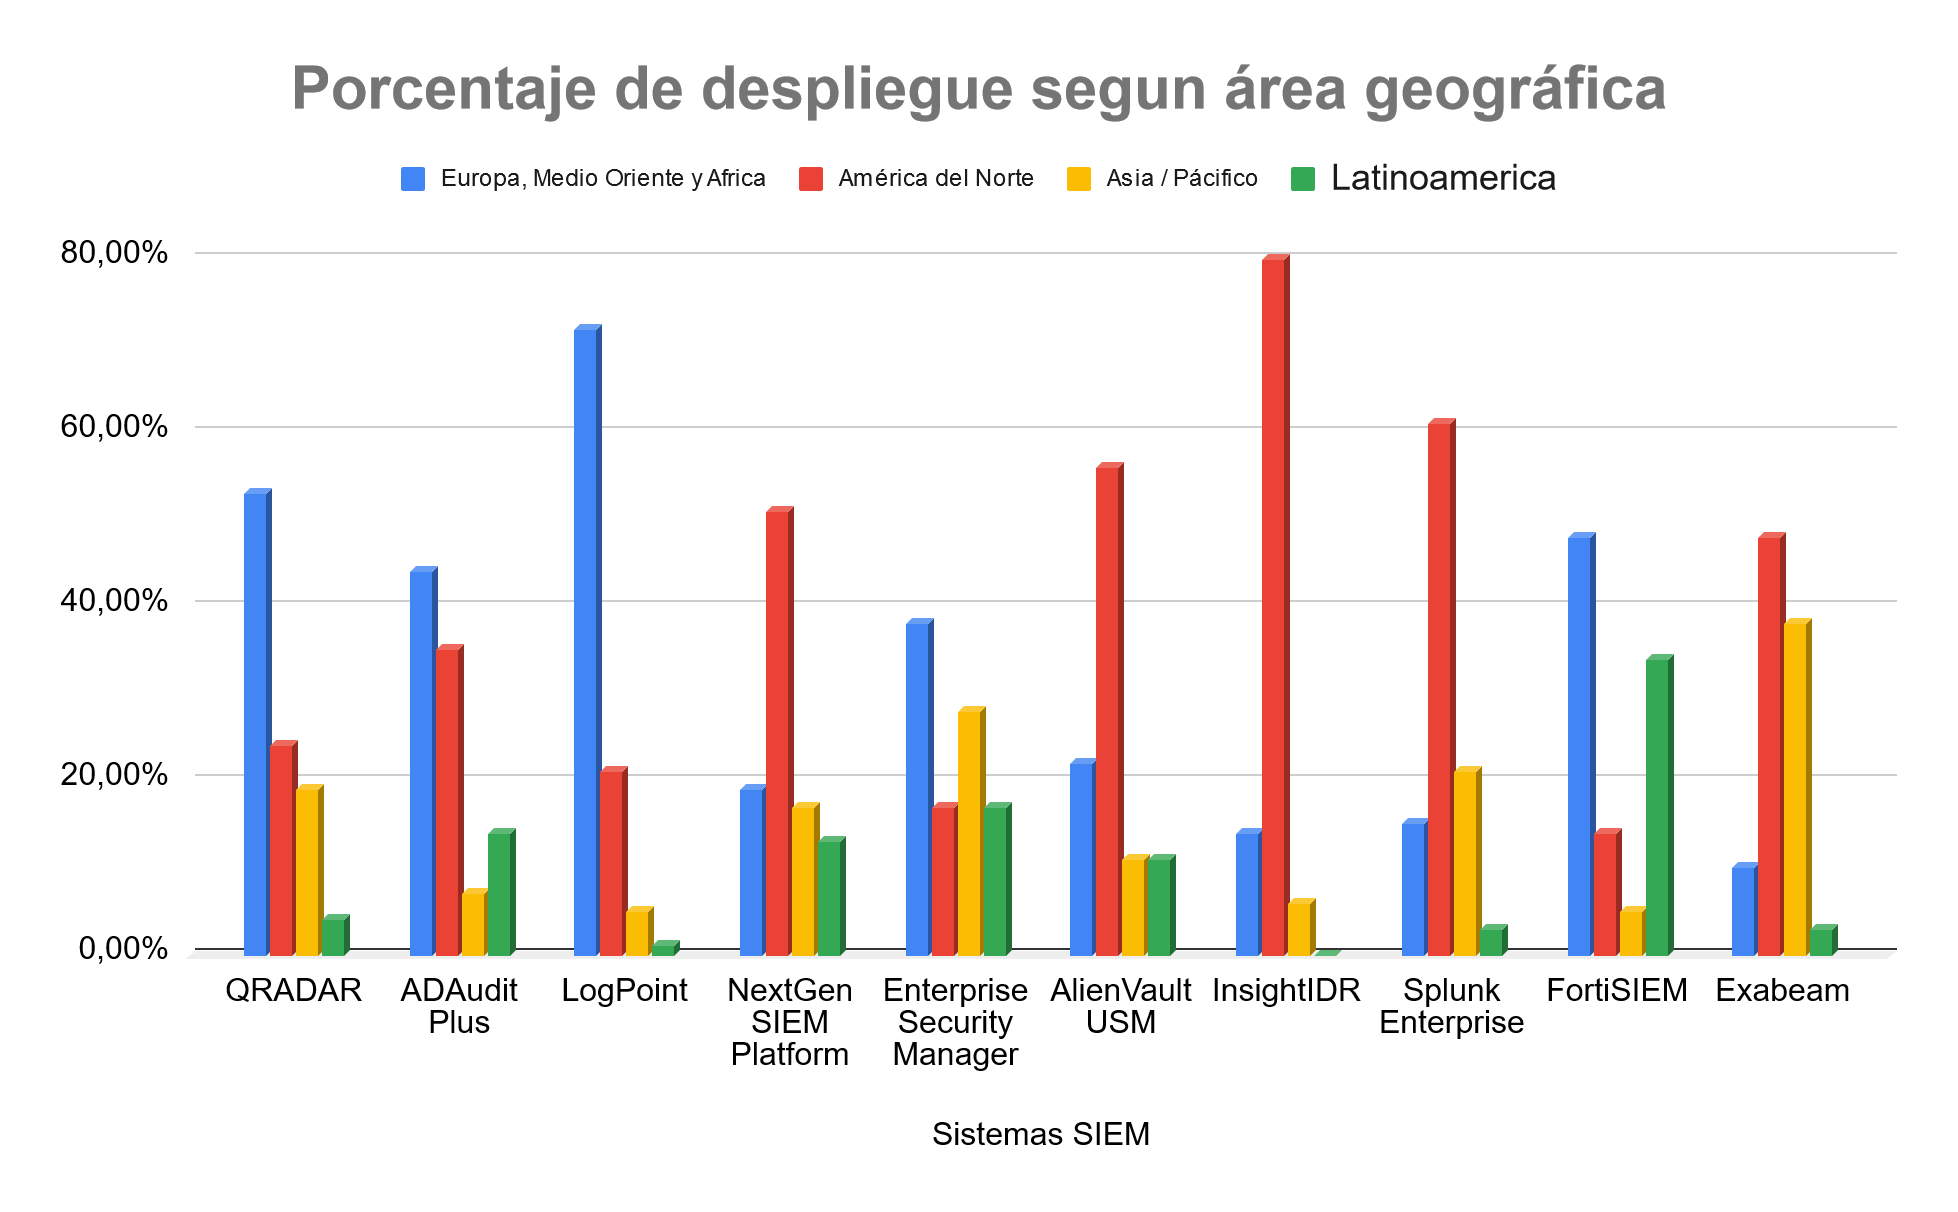
\includegraphics[width=1\textwidth]{./marco_teorico_imagenes/figura_11_porcentaje_area_geografica.png}
            \caption{Porcentaje de despliegue según área geográfica}
            \label{fig:area_geografica_mundial}
        \end{figure}
        \FloatBarrier
        \vspace{-0,5cm}
        En la Figura \ref{fig:area_geografica_mundial} se observa que las soluciones QRADAR\cite{qradar}, LogPoint\cite{logpoint} y FortiSIEM\cite{fortisiem} concentran su demanda en Europa, Medio Oriente y África. En el continente americano existe un contraste entre los mercados de América del Norte y de América Latina. En el norte del continente la mayor parte del mercado es atendido por las soluciones de Enterprise Security Manager\cite{enterprise}, InsightIDR\cite{insight} y AlienVault USM\cite{alienvault_usm}, mientras que la plataforma FortiSIEM es la preferida en Iberoamérica. \par
        \begin{figure}[H]
            \centering
            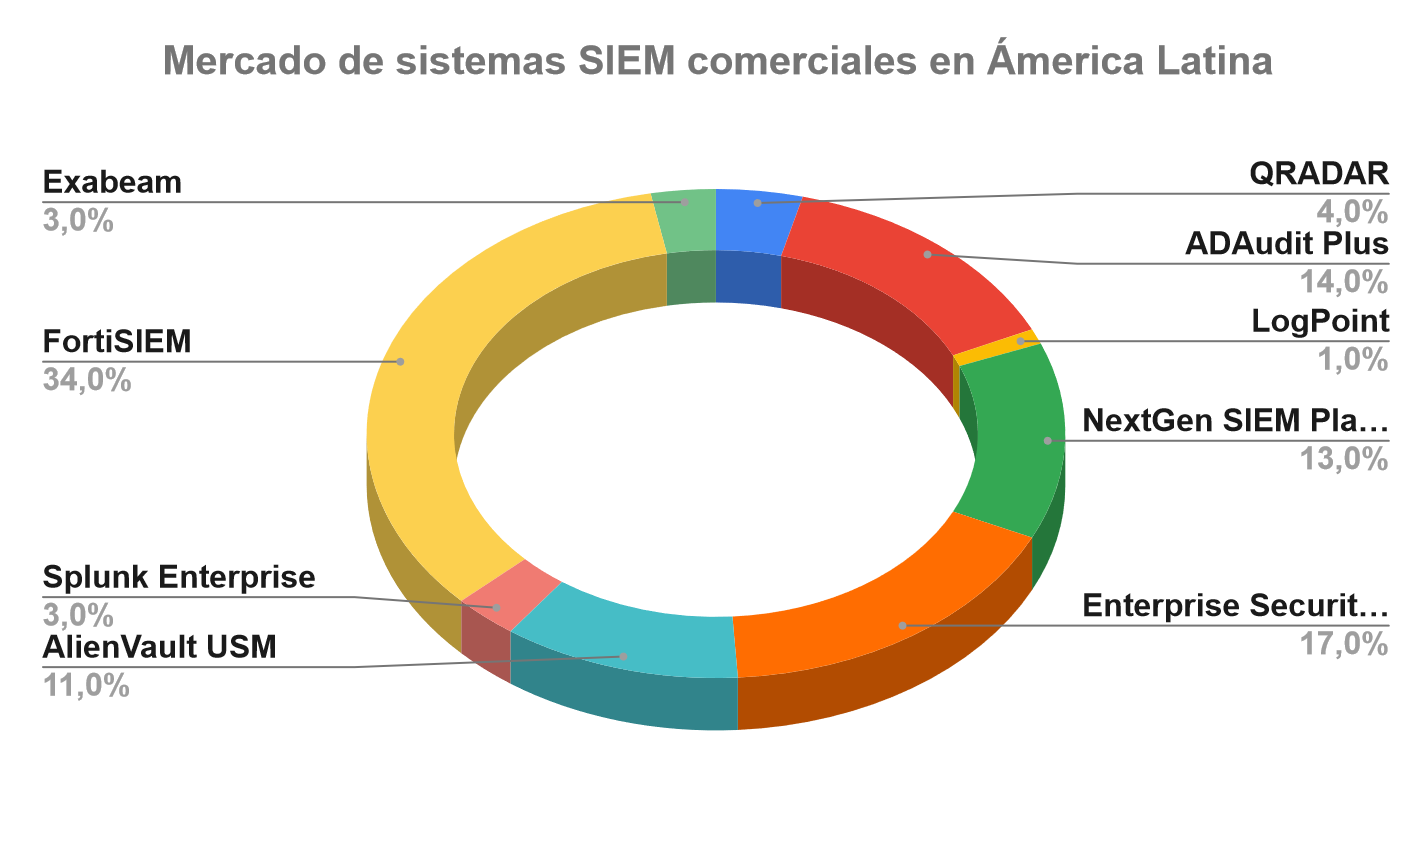
\includegraphics[width=1\textwidth]{./marco_teorico_imagenes/figura_12_comercial_america_latina.png}
            \caption{mercado de sistemas SIEM comerciales en América Latina}
            \label{fig:comercial_latam}
        \end{figure}
        \FloatBarrier
        Sobre nuestra región, en la Figura \ref{fig:comercial_latam} se observó que FortiSIEM acapara el 34 \% del mercado, seguido de Enterprise Security Manager, ADAudit Plus y NextGen SIEM Platform con un 17, 14 y 13 \% del mercado, respectivamente.
        \end{subsection}
        
        \begin{subsection}{Soluciones gratuitas y de código abierto}
        Como consecuencia del relevamiento de las soluciones libres que se encuentran disponibles, se observó que la oferta de productos que cubren estas necesidades es acotada. Incluso en algunos casos, hay proyectos que se encuentran en estado de abandono, como por ejemplo Sweet Security[39]. Este proyecto no cuenta con soporte desde el año 2017. Por otro lado, las versiones abiertas de productos propietarios presentan serias limitaciones respecto de su equivalente comercial, lo que dificulta su consideración como alternativa viable para una organización. \par
        Sin embargo, existen soluciones íntegramente libres capaces de cumplir adecuadamente las misiones de un SIEM, constituyendo una opción válida y competitiva frente a los principales productos comerciales.\par
        Al igual que en el caso de los productos comerciales, se realizó un análisis sobre los sectores industriales a nivel mundial donde predominan las soluciones gratuitas. Como resultado, se observó un uso intensivo en las áreas de servicios IT, esto se debe a que en estas áreas predominan empresas desarrolladoras de tecnología de la información y entes gubernamentales, por lo que en ambos casos cuentan con el personal y recursos necesarios para modificar las soluciones a la medida de sus objetivos e infraestructura. En la Figura \ref{fig:sector_industrial_sol_libre} se puede observar el porcentaje de adopción por área en la industria.\par
        
        \begin{figure}[H]
            \centering
            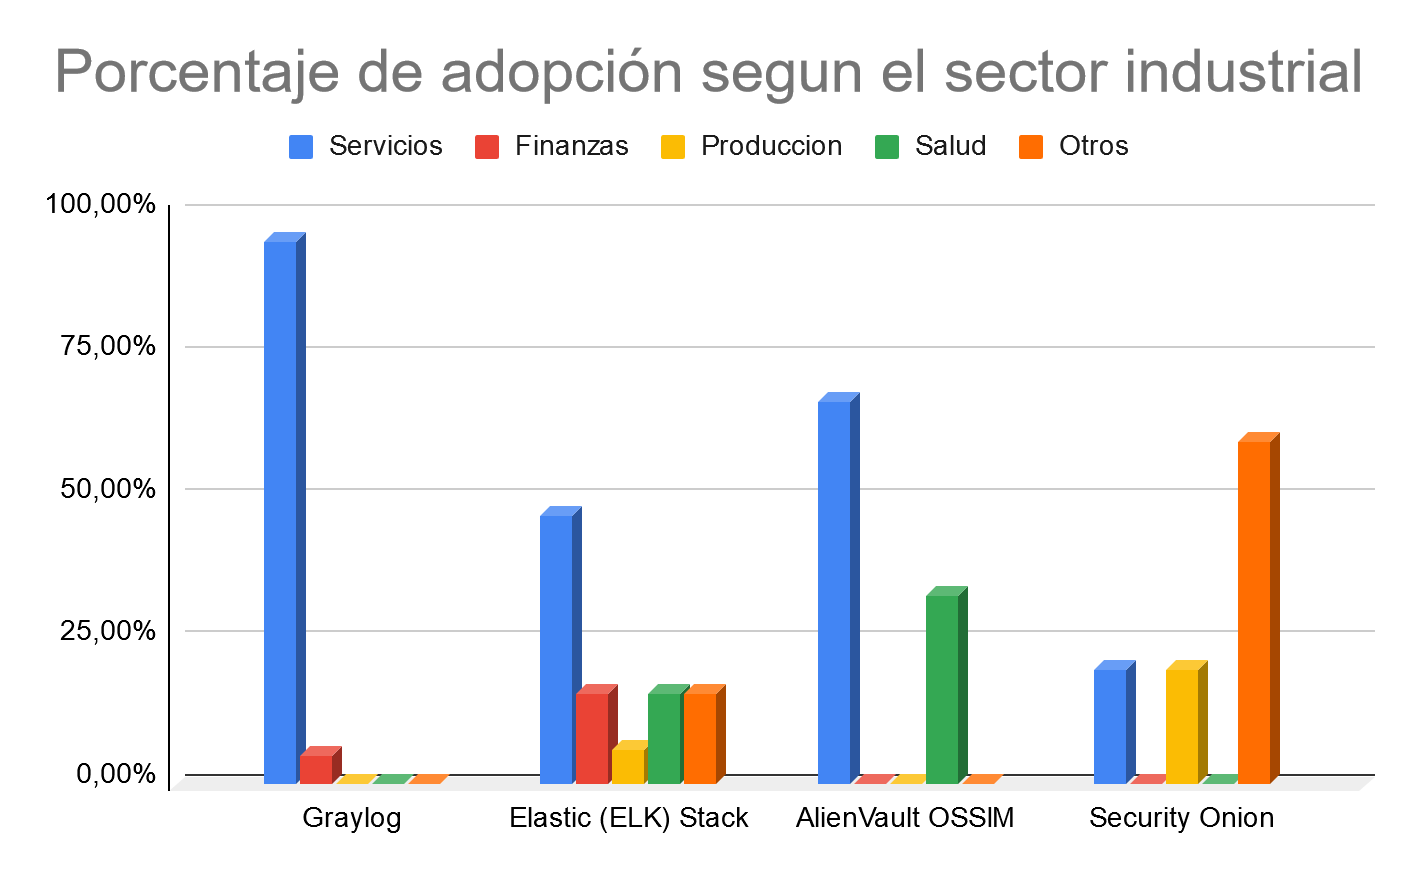
\includegraphics[width=1\textwidth]{./marco_teorico_imagenes/figura_13_ sol_libres_sector_ind.png}
            \caption{Porcentaje de adopción según el sector industrial para el caso de las soluciones libres. Gartner 2019 \cite{ranking}}
            \label{fig:sector_industrial_sol_libre}
        \end{figure}
        
        Por otro lado, se realizó el estudio de la región y el porcentaje de uso de las soluciones. Se observó que la pila Elastic tiene una presencia significativa en todas las regiones, como se puede ver en la Figura \ref{fig:region_implen_sol_libre}.\par
        
        \begin{figure}[H]
            \centering
            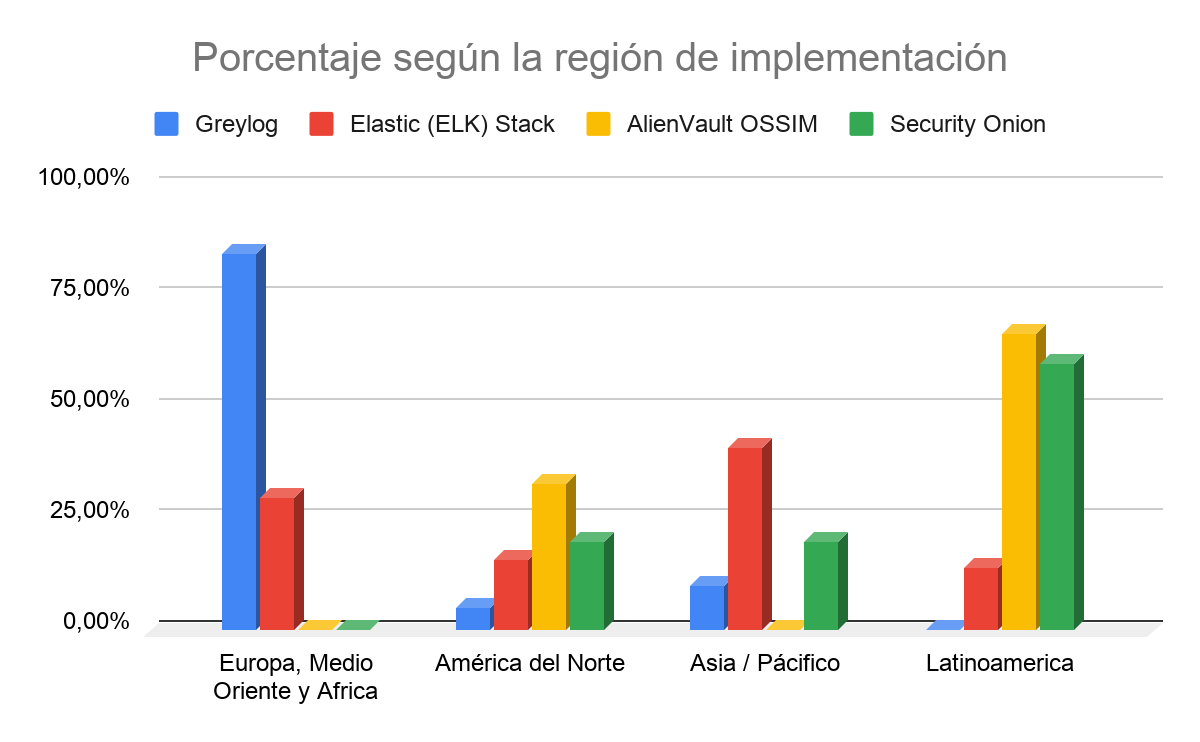
\includegraphics[width=1\textwidth]{./marco_teorico_imagenes/figura_14_region_implen_sol_libre.png}
            \caption{Porcentaje según la región de implementación}
            \label{fig:region_implen_sol_libre}
        \end{figure}
        
        Otra conclusión que se puede destacar del gráfico es que en América del norte y del sur la solución SIEM más utilizada es AlienVault OSSIM \cite{alienvault_ossim}, mientras que en Europa, Medio Oriente y África es Graylog \cite{graylog} así como en Asia/Pacífico optan por la pila Elastic\cite{elastic}.\par
        
            \begin{subsubsection}{AlienVault OSSIM}
            AlienVault OSSIM \cite{alienvault_ossim} es una solución desarrollada por la compañía estadounidense de telecomunicaciones AT \& T. Se trata de una alternativa libre a AlienVault USM, que es la solución comercializada por la empresa. Permite la recopilación, normalización y correlación de eventos, ofreciendo un subconjunto de las capacidades de la variante comercial. El fabricante recomienda esta solución para profesionales IT de organizaciones pequeñas y de pocos recursos, investigadores de seguridad y miembros de la comunidad académica. \par
            Sus capacidades de monitoreo incluyen entornos físicos y virtuales pero no permite un despliegue descentralizado, ya que solo admite la instalación en un único servidor. Entre sus limitaciones se cuentan la ausencia de gestión de logs y la capacidad de detección en puntos finales. A pesar de esto, es la solución SIEM más utilizada en América Latina.

            \end{subsubsection}
            \begin{subsubsection}{Graylog}
            Graylog \cite{graylog} es una solución SIEM desarrollada por la compañía del mismo nombre. Dispone de una arquitectura enfocada a la administración centralizada de logs y, a diferencia de otros sistemas, es capaz de recibir y procesar datos en distintos formatos tales como Syslog, NetFlow, JSON, entre otros. Permite una arquitectura de despliegue descentralizada, donde la recolección, normalización y correlación de eventos se llevan a cabo de manera centralizada. Utiliza una base de datos de elasticsearch y es una solución apta para escalar al tamaño que requiera cualquier organización. \par 
            Entre sus principales ventajas se encuentra su motor de procesamiento de logs, que permite consultar y procesar información de una manera más eficiente que otras soluciones disponibles. Otra de sus ventajas es la tolerancia a fallos, que previene la pérdida de datos en el caso de producirse algún problema de red. Esto facilita el almacenamiento distribuido de datos y el balanceo de carga en las bases de datos. Como se observa en la Figura \ref{fig:region_implen_sol_libre}, Graylog es la solución SIEM más utilizada en Europa, Medio Oriente y África.

            \end{subsubsection}
            \begin{subsubsection}{Elastic Stack}
            Elastic Stack\cite{elastic}, a diferencia de las soluciones descritas anteriormente, no constituye por sí mismo un SIEM como plataforma integral. Sin embargo, es utilizado como columna vertebral de muchos proyectos de software libre, código propietario y soluciones a medida debido a su capacidad de procesamiento de la información. \par
        	Elastic Stack se destaca por el soporte de mensajes provenientes de múltiples fuentes y despliegue de distintos tipos de arquitecturas. Como resultado, dispone de capacidades de almacenamiento tales como escalamiento de infraestructuras, alta disponibilidad, recuperación automática de réplicas y balanceo de carga, etc. En cuanto a la visualización cuenta con una GUI web que permite definir consultas e interactuar con los datos recibidos, mostrando los resultados de una manera intuitiva y visible. 

            \end{subsubsection}
            \begin{subsubsection}{Security Onion}
            Se trata de una distribución Linux basada en Ubuntu \cite{ubuntu} que cuenta con un suite de diversas herramientas dedicadas a la ciberseguridad. Utiliza la pila completa de Elastic Stack para la recopilación, procesamiento y visualización de la información. Admite distintos tipos de arquitectura de despliegue, permitiendo adaptar los recursos disponibles según las necesidades de una organización. Actualmente se encuentra en desarrollo y cuenta con el soporte activo de una comunidad. Es la solución elegida para el desarrollo de este proyecto integrador.
            \end{subsubsection}
            
        \end{subsection} 
    \end{section}
    \begin{section}{Corolario}
    El uso masivo de las tecnologías de la información, así como la convergencia e interconexión de redes y sistemas, ha generado nuevos tipos de riesgos y amenazas en las organizaciones. Los ataques han evolucionado en complejidad, sigilo y focalización de los objetivos, implicando de esta manera mayores esfuerzos para su detección y resolución. \par
	Las organizaciones, públicas y privadas, deben esforzarse en preservar la seguridad de sus activos de información y responder a los nuevos riesgos e incidentes. Esto lleva a la necesidad de desplegar soluciones del tipo CSIRT. \par
    La Universidad Nacional de Córdoba, por sus características como organización y teniendo en cuenta el panorama anteriormente descrito, no se encuentra exceptuada de posibles ciberataques contra sus activos de información. Por lo tanto, se encuentra justificada la creación de un CSIRT que atienda a sus propias necesidades. \par

    \end{section}
            
            
            
            
